\documentclass{article}

% Language setting
% Replace `english' with e.g. `spanish' to change the document language
\usepackage[italian]{babel}
\usepackage{float}
\usepackage{subfig}

% Set page size and margins
% Replace `letterpaper' with `a4paper' for UK/EU standard size
\usepackage[letterpaper,top=2cm,bottom=2cm,left=3cm,right=3cm,marginparwidth=1.75cm]{geometry}

% Useful packages
\usepackage{amsmath}
\usepackage{graphicx}
\usepackage{float}
\usepackage[colorlinks=true, allcolors=blue]{hyperref}

\setlength{\parskip}{6pt}%

\title{Simulatore del movimento dei pianeti in un sistema solare}
\author{Gioele Mancino, Federico Mastroforti, Luca Tesei, Nico Tortorici}

\begin{document}
\maketitle
\section{Introduzione}

\subsection{Obiettivo del simulatore}
Lo scopo del programma quello di simulare un sistema di N corpi planetari o stellari secondo la fisica newtoniana. L'obiettivo principale era quello di creare un sistema solare stabile, in grado cioè di preservare le orbite nel tempo, senza che queste degenerino.

Oltre all'obiettivo principale, si sono volute implementare altre funzionalità utili all'utente, tra cui:
\begin{itemize}
    \item finestra grafica per visualizzare i corpi, con relativa interfaccia grafica;
    \item possibilità di inserire nuovi corpi con una massa e direzione a scelta;
    \item possibilità di avviare, interrompere o ripristinare la simulazione;
    \item possibilità di scegliere tra diverse configurationi iniziali.
\end{itemize}

\subsection{Istruzioni per la compilazione}

Piattaforma di riferimento: Ubuntu 20.04.

Eseguire il pull della repository con il comando:
\begin{verbatim}
    $ git clone https://github.com/NexganGH/gravity_simulator
\end{verbatim}

Installare \href{https://www.sfml-dev.org/tutorials/2.5/start-linux.php}{SFML v2.5.1} con il comando:
\begin{verbatim}
    $ sudo apt-get install libsfml-dev=2.5.1+dfsg-1build1
\end{verbatim}

Installare \href{https://www.sfml-dev.org/tutorials/2.5/start-linux.php}{TGUI}, libreria estensione di SFML per create le interfacce utenti:
\begin{verbatim}
   $ sudo add-apt-repository ppa:texus/tgui
   $ sudo apt-get update
   $ sudo apt-get install libtgui-1.0-dev
    \end{verbatim}

Assicurarsi di avere CMake installato, da installare altrimenti con:
\begin{verbatim}
    $ sudo apt-get install cmake
\end{verbatim}

Il programma può essere compilato, \textit{per la release}, con:
\begin{verbatim}
    $ cmake -S. -B build -DBUILD_TESTING=Off -DCMAKE_BUILD_TYPE=Release
    $ cmake --build build
    $ build/gravity
     \end{verbatim}

Questo creerà un eseguibile \verb|gravity| nella cartella \verb|build|, da eseguire con il comando:
\begin{verbatim}
    $ build/gravity
\end{verbatim}

\subsection{Funzionalità}
Il programma consiste in uno spazio in cui sono presenti diversi corpi stellari, i quali sono soggetti a gravità reciproca.

La schermata iniziale prevede una simulazione del sistema solare fino a Marte. L'utente può da qui avviare la simulazione con il tasto in alto a sinistra. 

Tra le varie funzionalità:
\begin{itemize}
    \item l'utente può inserire un nuovo corpo con click destro del mouse. Questo tasto apre una finestra che richiede di inserire la massa \textbf{in unità terrestri} (1 = massa della Terra). Successivamente è richiesto scegliere la direzione verso cui il corpo verrà lanciato con una velocità di modulo 30 km/s.
    \item l'utente può mettere in pausa la simulazione
    \item l'utente può ripristinare la simulazione con il tasto "reset", in alto a sinistra.
    \item l'utente può scegliere tra varie configurazioni predefinite in alto a sinistra.
\end{itemize}

Altre caratteristiche:
\begin{itemize}
    \item la grandezza dei pianeti è proporzionale in maniera esponenziale alla massa (con esponente $< 1$);
    \item il colore dei pianeti è casuale; il colore delle stelle varia da giallo a rosso a seconda della massa.
    \item la finestra è sempre quadrata e dipende dalla grandezza dello schermo dell'utente.
\end{itemize}

Da notare che l'interfaccia grafica non scala con la grandezza dello schermo dell'utente.

\begin{figure} [H]
    \centering
    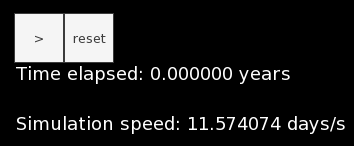
\includegraphics[height=.20\linewidth]{Playpause.png}
    \captionof{figure}{Il tasto (sinistra) Play/Pause permette di far partire e fermare la simulazione in ogni momento, mentre il tasto (destra) reset riporta la simulazione allo stato iniziale  (i corpi già presenti ritornano nel punto in cui erano a inizio simulazione mentre quelli generati dall’utente vengono eliminati) }
    \label{playpause}
\end{figure}

\begin{figure} [H]
    \centering
    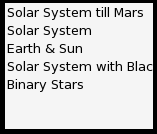
\includegraphics[height=.20\linewidth]{menu.png}
    \captionof{figure}{Il menù presente nella parte alta a sinistra dell'interfaccia serve a selezionare delle simulazioni prefabbricate. Cliccandone una essa comparirà nello schermo.}
    \label{menu}
\end{figure}

\subsection{La fisica dietro al programma}
\label{fisica}
La legge di gravitazione universale afferma che due punti materiali si attraggono con una forza di intensità direttamente proporzionale al prodotto delle masse dei singoli corpi e inversamente proporzionale al quadrato della loro distanza. Questa legge, espressa vettorialmente, diventa:
\begin{equation}
    \mathbf{F}_{2,1}(\mathbf{r})=-\frac{Gm_{1}m_{2}}{r^{2}}\mathbf{\hat{u}}_{r}
\end{equation}
dove $\textbf{F}_{2,1}$ è la forza con cui l'oggetto 1 è attratto dall'oggetto 2, G è la costante di gravitazione universale, che vale circa $6,67\cdot 10^{-11}\frac{Nm^2}{kg^2}$, $m_1$ e $m_2$ sono le masse dei due corpi, $\textbf{r}=\textbf{r}_1-\textbf{r}_2$ è il vettore congiungente i due corpi (supposti puntiformi), 
$r$ è il suo modulo e $\hat{\textbf{u}}_{r}=\frac{\textbf{r}}{r}$ rappresenta il versore che individua la retta congiungente i due punti materiali.

Il programma utilizza questa relazione per calcolare istante per istante le forze che agiscono su ogni corpo, e di conseguenza le accelerazioni:
\begin{equation}
    \textbf{F}_{j,tot}=\sum_{i=1, i\neq j}^{N_{bodies}}\textbf{F}_{i}(\textbf{r})=m\ddot{\textbf{r}}_{j,tot}
    \label{eq2}
\end{equation}
dove $\textbf{F}_{j,tot}$ è la forza risultante che agisce sul corpo $j$.

Integrando poi la precedente equazione si ottiene la legge oraria $\textbf{r}(t)$ del corpo $j$. Non essendo risolvibile analiticamente si deve ricorrere a metodi di integrazione numerica.

\section{Trattazione matematica}
Siccome la forza gravitazionale è una grandezza vettoriale (vedi \ref{fisica}) è possibile scomporla nelle sue due componenti indipendenti\footnote{Il progetto infatti tratta solo il caso bidimensionale.}: nel caso del progetto si è preferito fare utilizzo delle coordinate cartesiane, così da poter ottenere, a partire dalla \ref{eq2}, le equazioni differenziali qui sotto riportate, le cui soluzioni descrivono rispettivamente la proiezione sull'asse x ed y del moto dei corpi.

\begin{equation}
    F_{j,x,tot}=\sum_{i=1,i\neq j}^{N_{bodies}}-\frac{Gm_{j}m_{i}}{d_{j,i}^2}\frac{x_{j}-x_{i}}{d_{j,i}}=m_{j}\ddot{x_{j}}
    \label{eq3}
\end{equation}
\begin{equation}
    F_{j,y,tot}=\sum_{i=1,i\neq j}^{N_{bodies}}-\frac{Gm_{j}m_{i}}{d_{j,i}^2}\frac{y_{j}-y_{i}}{d_{j,i}}=m_{j}\ddot{y_{j}}
\label{eq4}
\end{equation}
dove $F_{j,x,tot}$ e $F_{j,y,tot}$ sono le componenti cartesiane della forza totale che agisce sul corpo $j$, $x_{j}, x_{i}$ e $y_{j}, y_{i}$ sono rispettivamente le ascisse e le ordinate dei corpi $j$ e $i$, $\ddot{x_{j}}$ e $\ddot{y_{j}}$ sono le componenti cartesiane dell'accelerazione del corpo $j$, $d_{j,i}$ è la distanza tra i due corpi, così definita:
\begin{equation}
    d_{j,i}=\sqrt{(x_{j}-x_{i})^2+(y_{j}-y_{i})^2}
\end{equation}
Le equazioni \ref{eq3} e \ref{eq4} possono essere scritte in forma vettoriale, ottenendo:
\begin{equation}
    \textbf{F}_{j,tot}=\sum_{i=1,i\neq j}^{N_{bodies}}-\frac{Gm_{j}m_{i}}{d_{j,i}^2}(\frac{x_{j}-x_{i}}{d_{j,i}}; \frac{y_{j}-y_{i}}{d_{j,i}})=m_{j}(\ddot{x_{j}}; \ddot{y_{j}})
\label{eq5}
\end{equation}
dove $(\frac{x_{j}-x_{i}}{d_{j,i}}; \frac{y_{j}-y_{i}}{d_{j,i}})$ è il versore del vettore distanza tra i due corpi\footnote{Si veda la trattazione matematica in appendice \ref{ap1}}.

Nel progetto si farà uso di questa equazione in forma vettoriale, alla quale verranno appliacati i metodi di integrazione numerica che ci proponiamo di trattare di seguito.
\subsection{Metodo LeapFrog}
Come precedentemente menzionato, la soluzione dell'equazione differenziale \ref{eq5} per ogni singolo corpo risulta impossibile da ricavare analiticamente. Si deve quindi ricorrere a metodi numerici di integrazione per equazioni differenziali.
Nel presente progetto,  per ottenere la posizione $\mathbf{r}_{j}$ e la velocità $\mathbf{\dot{r}}_{j}$ del corpo $j$(\footnote{Il sistema di riferimento utilizzato è quello della finestra grafica nel quale  l'origine è posta nel vertice in alto a sinistra, l'asse delle ascisse positivo verso destra e quello delle ordinate positivo verso il basso.}), che risente dell'attrazione gravitazionale simultanea degli altri N-1 corpi,è stato adottato il metodo Leapfrog.
È un sistema ampiamente utilizzato per ricavare numericamente le soluzioni di equazioni differenziali scalari del tipo:
\begin{equation}
    \ddot{x}=\dot{v}=A(x)
\end{equation}
L'algoritmo permette di calcolare la posizione del corpo in esame allo step $i+1$ $x_{i+1}$ nota la positione allo step $i$ $x_{i}$ e la velocità del corpo allo step $v_{i+\frac{1}{2}}$.

Le equazioni per aggionare la posizione e la velocità del corpo al rispettivo step sono:
\begin{equation}
    v_{i+\frac{1}{2}}=v_{i}+\frac{1}{2}a_{i}\Delta t
\end{equation}
\begin{equation}
    x_{i+1}=x_{i}+v_{i+\frac{1}{2}}\Delta t
\end{equation}
\begin{equation}
    v_{i+1}=v_{i+\frac{1}{2}}+ \frac{1}{2}a_{i+1}\Delta t
\end{equation}
dove $a_{i}=A(x_{i})$.

Il suddetto metodo integrativo ha la proprietà di conservare l'energia meccanica totale, risultando in una completa stabilità delle orbite dei corpi (vedi confronto in appendice con altri metodi testati per l'implementazione \ref{ap2}) e per questo motivo viene specialmente utilizzato per simulare, come nel presente caso, le traiettorie coniche dei pianeti.

\section{Implementazione}
\subsection{Strumenti utilizzati}
È stato utilizzato C++ 17, compilator tramite GCC.

Si sono utilizzate le librerie:
\begin{itemize}
    \item SFML 2.5.1 per l'implementazione grafica.
    \item \href{https://tgui.eu/tutorials/1.0/linux/}{TGUI 1.0} per l'interfaccia utente.
\end{itemize}

Per il linking dei file e la creazione degli executable, come i test, è stato usato CMake 3.16.

Per lo sviluppo è stato utilizzato l'IDE Visual Studio Code, usato in ambiente WSL con Ubuntu 20.04. È stato adottato, per la formattazione, un file \href{https://github.com/NexganGH/gravity_simulator/blob/master/.clang-format}{.clang-format} basato sullo stile di Google.

Per effettuare il controllo delle versioni, è stato utilizzato Git 2.5.1; come repository remota è stato adottato GitHub. La repository è presente al link: \url{https://github.com/NexganGH/gravity_simulator/tree/master}


\subsection{Struttura dei file}
La directory principale contiene è divisa nelle seguenti sotto-directory:
\begin{itemize}
    \item \verb|docs/| contiene questo file, il suo sorgente in Latex e altri file necessari alla compilazione.
    \item \verb|include/| contiene gli header (\verb|.hpp|).
    \item \verb|src/| contiene i file \verb|.cpp| con le definizioni.
    \item \verb|test/| contiene i file di testing.
\end{itemize}

\subsection{Struttura generale delle classi}

L'obiettivo di design del progetto è stato quello di sfruttare al massimo la OOP per garantire la massima riusabilità delle classi, in egual modo aumentando la mantenibilità e scalabilità del codice.

La classe cardine del programma è \verb|SimulationState|, la quale rappresenta lo stato corrente della simulazione. Essa contiene:
\begin{itemize}
    \item la lista dei corpi presenti nello spazio (vettore di \verb|Body|);
    \item un'istanza di \verb|Configuration|, che rappresenta la configurazione iniziale attualmente in uso;
    \item un'istanza di \verb|PhysicsEngine|, classe che si occupa di effettuare i calcoli circa le posizioni dei pianeti;
    \item un'istanza di \verb|Renderer|, il cui scopo è disegnare a schermo i pianeti.
\end{itemize}

\verb|Body| è una classe che rappresenta un corpo nello spazio, dotato di una posizione, velocità, forza e massa. Tale classe è astratta poiché alcuni metodi dipendono dal tipo del corpo, distinzione eseguita tramite ereditarietà (attualmente le classi figlie sono \verb|Planet| e \verb|Star|).

\verb|Configuration| rappresenta uno specifico stato iniziale della simulazione: è quindi caratterizzato da una lista di corpi con le loro posizioni iniziali. A tal propositio, la funzione \verb|getConfigurations| fornisce una lista di configurazioni, le quali sono mostrate all'utente in alto a sinistra nell'interfaccia.

\verb|PhysicsEngine| è la classe che esegue i calcoli: il suo metodo pubblico più importante è \verb|evolve|, il quale permette di evolvere una lista di corpi nell'arco di tempo \verb|dt|. Esso implementa il metodo di integrazione LeapFrog.

\verb|Renderer| è la classe che permette di disegnare a schermo i corpi e i componenti dell'interfaccia. Nel caso dei corpi, è effettuata un automatico una conversione dalle coordinate dei corpi, espressi in coordinate reali (metri), alle coordinate sullo schermo (pixel). Tale conversiene avviene, ovviamente, in base alla larghezza dell'universo in visione (variabile a seconda della configurazione).

\verb|GuiManager| è una classe che crea e gestisce l'interfaccia utente.

\subsection{PhysicsEngine}
\label{physics_engine}
Il metodo principale, \verb|evolve|, oltre ha come parametro la lista dei corpi da evolvere e l'intervallo di tempo \verb|dt|. Tale intervallo deve corrispondere all'intervallo di tempo che è trascorso \textit{nella realtà} dalla scorsa chiamata di \verb|evolve|.

Al fine di simulare eventi che avvengono in periodi estesi, come anni, è necessario però utilizzare una \verb|timescale|, ovvero un valore che velocizzi la simulazione. Tale valore è moltiplicato per il \verb|dt| del metodo evolve. Si incorre nella seguente relazione:

\begin{equation*}
    T_{simulazione} = n \cdot dt \cdot timescale
\end{equation*}

dove $T_{simulazione}$ è il tempo trascorso, in secondi, nella simulazione durante $n$ chiamate di \verb|evolve| di un intervallo di tempo $dt$ ciascuno.

 Se $n \cdot dt = 1 s$, cioè è passato 1 secondo nella realtà, si ha che $T_{simulazione} = timescale$; da ciò si conclude che timescale, espresso in secondi, rappresenta il numero di secondi passato nella simulazione durante un secondo nella realtà.

Si noti inoltre che, siccome $dt$ dipende dalla velocità con cui viene eseguito il ciclo, quindi dall'hardware dell'utente, il tempo della simulazione è normalizzato: \textit{la velocità della simulazione è costante in tutti gli ambienti/dispositivi}.

Questo implica il fatto, però, che un utente con un hardware lento, a parità di timescale, avrà degli intervalli di calcolo maggiori, diminuendo l'accuratezza dei calcoli. A tal proposito può essere ridotto il timescale.

\subsection{Renderer}
La classe \verb|Renderer| ha lo scopo di disegnare i corpi e l'interfaccia a schermo. Poiché le posizioni dei corpi sono espressi in coordinate reali (metri), è necessario che prima di disegnarli a schermo le loro coordinate sono convertite. A tal proposito, il metodo statico \verb|fromUniverseWidth| permette di calcolare una scala a partire dalla grandezza dell'universo e della finestra:
\begin{equation*}
    scale = \frac{universe\;width}{window\;width}
\end{equation*}

Per convertire una coordinata \verb|x| da coordinate reali a coordinate sullo schermo, si usa la relazione:
\begin{equation*}
    x_{schermo} = \frac{x_{reale}}{scale}
\end{equation*}

\subsection{Configuration}
La classe \verb|Configuration| contiene lo stato iniziale del progetto - tra cui la lista dei corpi. Lo scopo della classe è quello di fornire gli elementi per inizializzare \verb|SimulationState|. La lista dei corpi è fornita tramite copia, in modo che la lista all'interno della classe rimanga non modificata possa essere riutilizzata per il tasto "reset".

Sono state create diverse istanze di \verb|Configuration| per proporre diverse configurazioni iniziali all'utente. Queste sono istanziate nel metodo \verb|getConfigurations|.

\subsection{Altre classi}
Tra le altre classi del programma ci sono:
\begin{itemize}
    \item \verb|GuiManager|, utilizzata per la creazione e gestione dell'interfaccia.
    \item \verb|Vector|, utilizzata per rappresentare un vettore nello spazio 2D. Sono disponibili diverse operazioni.
    \item \verb|OrbitDrawer|, utilizzata per disegnare le orbite e cancellare i punti dopo un intervallo di tempo.
\end{itemize}

\subsection{Ciclo principale}
Il ciclo principale si svolge nel \verb|main|. Un ciclo permette di utilizzare il metodo \verb|evolve| di PhysicsEngine per evolvere la simulazione per un tempo indefinito. Il valore \verb|dt|, da fornire a \verb|PhysicsEngine| (si veda Sezione (\ref{physics_engine})), è misurato tramite un cronometro.

\subsection{Utilizzo dei puntatori}
Al fine di evitare memory leaks, sono stati utilizzati gli smart pointer. Ove possibile, è stato adottato lo \verb|unique_ptr|.

A titolo esemplificativo si consideri la lista di puntatori a \verb|Body|:
\begin{verbatim}
    std::vector<std::unique_ptr<Body>> _bodies;
\end{verbatim}

Il vettore contiene dei puntatori a \verb|Body| poiché questa è una classe astratta, si tratta quindi di polimorfismo dinamico.

\verb|Configuration| ne crea una copia che viene passata a \verb|SimulationState|. Per la copia si utilizza il metodo astratto di \verb|clone| che ritorna uno \verb|unique_ptr| all'oggetto \verb|Body| clonato: a questo punto viene creato un nuovo vettore con questi puntatori. L'ownership è poi passata a \verb|SimulationState|; tale principio è applicato anche agli altri puntatori all'interno di \verb|SimulationState|, la quale ne detiene l'ownership.

Per accedere ad un oggetto detenuto da \verb|SimulationState|, questa fornisce come interfaccia una serie di metodi che ritornano referenze agli \verb|unique_ptr|.

Per istanziare i puntatori si utilizzano i metodi \verb|std::make_unique| e \verb|std::make_shared|.

\section{Testing e debugging}
\subsection{Tecnica di testing}
È stato utilizzata la libreria \verb|doctest| per effettuare i testing. CMake permette di effettuare i linking e creare un eseguibile per ogni file di test.

\subsection{Eseguire un test}
I test sono contenuti in executable separati con il nome della classe.t. Ad esempio, per effettuare il test della classe \verb|PhysicsEngine|:
\begin{verbatim}
    $ cmake -S. -B build -DBUILD_TESTING=On
    $ cmake --build build --target physics_engine.t
    $ build/gravity
\end{verbatim}

Per eseguire i test, eseguire \verb|physics_engine.t| nella cartella \verb|build|:
\begin{verbatim}
    $ build/physics_engine.t
\end{verbatim}
\subsection{Memory Leak}
Durante i test non sono stati riscontrati memory leak provenienti dal codice originale. In determinati test si sono evidenziati, però, dei leak provenienti da SFML oppure TGUI la cui causa è sconosciuta.

\section{Risultati e problemi riscontrati}
Tramite il metodo Leapfrog, si è ottenuta con successo una simulazione in scala del sistema solare (fino a Marte oppure fino Nettuno a seconda della configurazione). 
Si riscontra, con successo:
\begin{itemize}
    \item che le orbite sono stabili e non degenerano nel tempo: ricoprono sempre lo stesso percorso;
    \item che la Terra rivoluziona attorno al Sole in 1 anno, come atteso;
    \item che le funzionalità implementate, come la creazione di un nuovo pianeta, il reset, la pausa funzionano correttamente;
    \item che la simulazione risulta anche in altri casi coerente con ciò che approssimativamente ci si aspetta.
\end{itemize}

Tra i problemi riscontrati, tuttavia, si evidenzia:
\begin{itemize}
    \item un peggioramento delle performance nel tempo, dovuto alla creazione dei punti delle orbite (anche se questi vengono cancellati dopo un certo periodo);
    \item dopo un periodo di simulazione elevato, il tempo di rivoluzione della Terra aumenta la proprio durata ($> 1$ anno). Si ipotizza che tale problema sia dovuto alle approssimazioni numeriche effettuate.
\end{itemize}

\appendix
\section{Calcoli e approssimazioni}
\subsection{Versore distanza tra due corpi}
\label{ap1}
Dati due corpi $p_{1}$ e $p_{2}$, si definisce il vettore distanza tra di essi come $\textbf{d}$:
\begin{equation}
    \textbf{d}=(x_{1}-x_{2}; y_{1}-y_{2})
\end{equation}
Per calcolare il suo versore è sufficiente riscalare lo stesso per l'inverso della sua norma:
\begin{equation}
    d=\sqrt{(x_{1}-x_{2})^2+(y_{1}-y_{2})^2}
\end{equation}
Di conseguenza la formula del versore distanza sarà:
\begin{equation}
    \mathbf{\hat{d}}=(\frac{x_{1}-x_{2}}{\sqrt{(x_{1}-x_{2})^2+(y_{1}-y_{2})^2}}; \; \frac{y_{1}-y_{2}}{\sqrt{(x_{1}-x_{2})^2+(y_{1}-y_{2})^2}})   
\end{equation}
Ecco perchè nel testo ci si riferisce alle sue componenti nella forma:
\begin{equation}
    \mathbf{\hat{d}}_{x}=\frac{x_{1}-x_{2}}{\sqrt{(x_{1}-x_{2})^2+(y_{1}-y_{2})^2}} ;\; \mathbf{\hat{d}}_{y}=\frac{y_{1}-y_{2}}{\sqrt{(x_{1}-x_{2})^2+(y_{1}-y_{2})^2}}
\end{equation}

\begin{figure} [H]
    \centering
    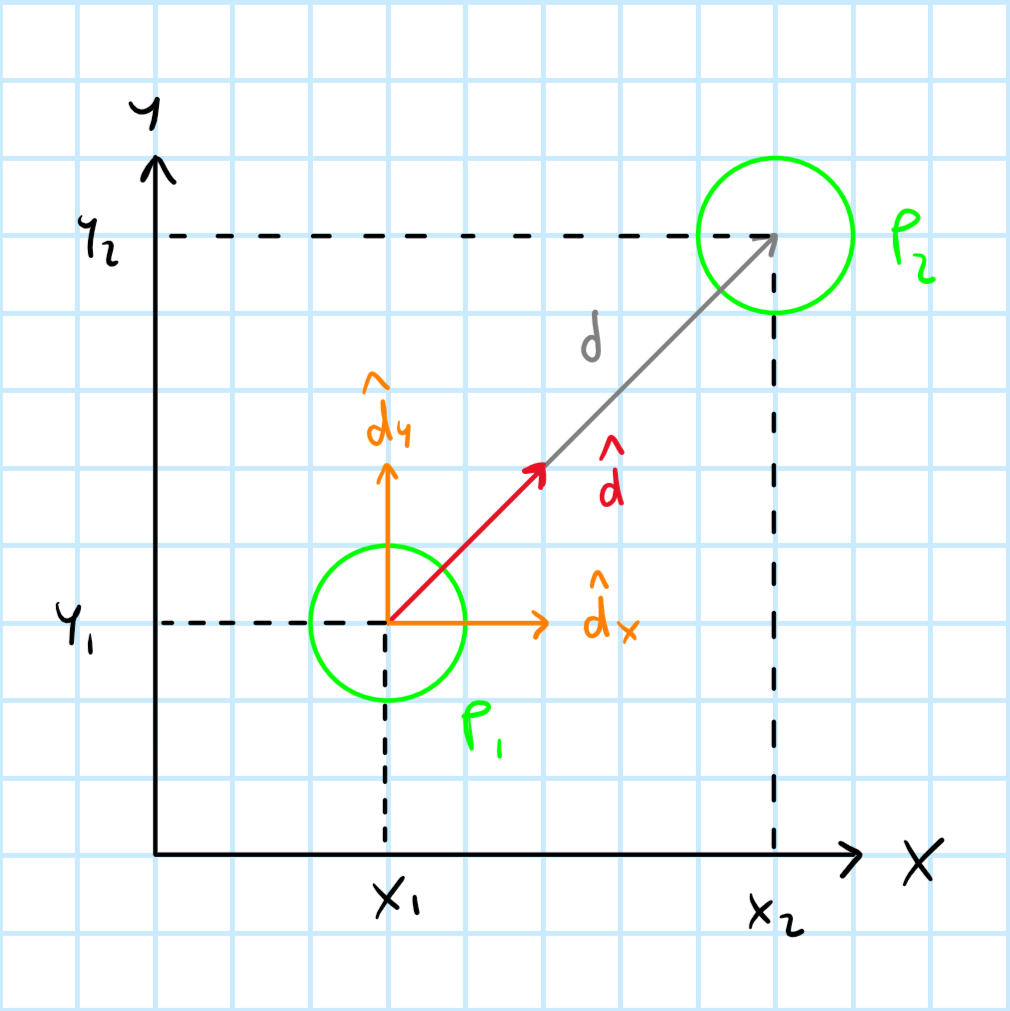
\includegraphics[height=.20\linewidth]{VersoreDistanza.png}
    \caption{Scomposizione in coordinate del versore distanza.}
\end{figure}


\subsection{Altri metodi di approssimazione}
\label{ap2}
Tra i vari metodi di integrazione numerica testati, il metodo LeapFrog si è rivelato il più accurato, mostrando una stabilità delle orbite notevolmente superiore a quella ottenuta con gli altri metodi.

La prima versione del progetto presentava un'implementazione del metodo di Eulero, basato sullo sviluppo in serie di Taylor, fino a terzo e quarto ordine. Le orbite erano instabili e divergevano.
\end{document}